\documentclass{scrartcl}
\usepackage[utf8]{inputenc}

\title{Modern Computer Architecture\\Literature Study}

\subtitle{Parallel programming and many-core architectures: where are the challenges?}

\author{%
    Mick van Gelderen\\4091566
    \and
    Arian Stolwijk\\4001079
}

\date{November 2013}

\usepackage{natbib}
\usepackage{graphicx}
\usepackage{listings}
\usepackage{color}
\usepackage{hyperref}

\hypersetup{%
    pdfauthor={Mick van Gelderen and Arian Stolwijk},
    pdftitle={Parallel programming and many-core architectures: what are the challenges?},
    colorlinks=false,
    hidelinks=true
}

\begin{document}

\maketitle

\begin{abstract}
    Since 2002 the way to increase performance is by using multiple cores and
    the number of cores keeps increasing. Utilizing the full potential of the
    entire processor in a parallel way is very difficult for programmers. This
    paper discusses various papers that describe parallel programming models
    that are designed helping programmers to increase the performance of their
    programs. Finally we've compared the solution by performance, ease of use
    and scaling.
\end{abstract}

\section{Introduction}

The assignment for this report was basically, find a kernel function from an
application and run it on the \rvex{}. To do this there are a few things we
need to know first:

\paragraph{Platform} The platform the program will run on is the ERA platform.
It consists out of the host processor, the MicroBlaze, accelerated with a
VLIW co-processor, the \rvex{}. For the co-processor computationally intensive
kernels can be extracted to achieve a performance increase.

\paragraph{Kernel function} The extracted piece of code is called the kernel.
The kernel needs to be compiled for the \rvex{} so that we can inject the
result, the bytecode, in to the co-processor. The rest of the code runs as
usual on a regular processor.

\paragraph{x264} The x264 program is the application we will try to improve
using the \rvex{}. x264 is a software library for encoding video streams
in the H.264 compression format.

The goal for this report is to extract the correct kernel, using profiling and
compile this for the \rvex{}. To execute the kernel on the \rvex{} there should
be communication between the processor and the co-processor.

\section{Discussion of different papers} \label{papers}

To investigate parallel programming for many-core architectures we've
considered four papers by different authors. The papers discus different
parallel programming methods or provide their own parallel programming
solution. The following sections each summarize a paper.

\subsection{Performance Analysis of Current Parallel Programming Models for Many-core Systems}

\emph{Performance Analysis of Current Parallel Programming Models for Many-core
Systems} \cite{CaoPerformanceAnalysis} is a paper written by Yangjie Cao et
al.\ in 2013.

%Nowadays processors consist out of many general purpose cores, and this will
%only increase. This kind of processors is usually referred to as many-core
%processors. Exploiting all the advantages of many-core processors however is
%not trivial.
%
%The shift to multi-core and many-core is a result of power consumption, heat
%dissipation and increasing processor frequencies.  In the near future it will
%be common to have a processor consisting hundreds or even thousands of cores.

To solve problems faced by many-core processor systems, extensive and intensive
research is carried out on parallel programming models. A good programming
model is usually judged on its generality. A good programming model can provide
an essential bridge between hardware and high-level programming languages.

%Programming models can be divided into two kinds: \emph{data-parallel} and
%\emph{task-parallel} programming models. Data-parallel focusses on solving
%data-independent problems and trying to distribute data on different parallel
%computing nodes. With task-parallel programmers focus on decomposing the
%problem into sub-tasks that can run in parallel.

Task-parallel programming is becoming increasingly popular in the last decade.
Several task-parallel libraries have been developed. These libraries allow
programmers to easily generate parallel tasks by handling how the
parallelization is realized on the underlying hardware.  Task scheduling and
load balancing are transparently completed by the runtime systems.

There are three typical task-parallel programming models described: Intel
Thread Building library (TBB), MIT Cilk and OpenMP 3.0. Several experiments are
done in order to compare these programming models.

Cilk is a task-based parallel programming model language. Cilk philosophy is
that the programmer can expose parallelism using a few keywords, while the Cilk
runtime does the hard work of scheduling the computation to run efficiently on
a given platform. The only addition to the programming language are three
keywords: \texttt{cilk}, \texttt{spawn} and \texttt{sync}.

TBB is a parallel programming library developed by Intel. It is mainly used the
way of task instead of thread to express parallelism. The library can map the
task efficiently on threads. TBB is a library so does not require special
languages or an extra compiler. TBB tasks are a special kind of C++ objects,
which allows the TBB model to explore a variety of parallelism. It supports
nested parallelism, so you can build larger parallel components.

OpenMP, which stands for Open Multiprocessing, was published by a group of
major hardware and software vendors. It gives programmers a simple and flexible
interface for developing parallel applications. The main aim is to simplify
programming of multi-platform, shared-memory, parallel programs by insertions
of pragmas into C/C++ code or special comments in Fortran code. These
insertions instruct the compiler which code should be parallelized. In the view
of OpenMP, tasks are units of work which are executed in parallel. A
disadvantage of OpenMP is that it lacks fine grained control.

To compare the different parallel programming models the authors conducted
experiments to evaluate and compare the performance of different models. There
were different benchmarks used (each model has different benchmarks). The
experiments were conducted on real many-core systems.

From experiment results most test applications obtain different levels of
performance speedup. Most applications achieve linear speedup when the number
of cores are increased. However when the number of cores is increased further,
the speedup becomes slower or even decreases.

The authors conclude that parallel programming models are crucial for
easy-to-understand, concise and dense representation of parallelism. The
experiments show that there are still many problems: (a) with scaling to
many-core systems, (b) low utilization and (c) resource competition.

\subsection{Parallel Phase Model: A programming Model for High-end Parallel Machines with Manycores}

\emph{Parallel Phase Model: A programming Model for High-end Parallel Machines
with Manycores} \cite{BrightwellParallelPhaseModel} is a paper written by
Ron Brightwell et al.\ in 2009.

Distributed parallel programming has mostly been done using the message passing
model, such as MPI\@. This has been very successful but still require programmers
to handle low-level tasks including explicit management of data distribution,
data locality management, communication preparation and scheduling,
synchronization and load balancing in order to achieve good performance.
With the introduction of multi-core and many-core machines will make developing
applications even more difficult because there will be node-level parallelism
and cluster-level parallelism.

A parallel programming model provides abstractions for programmers to express
parallelism and exploiting the capabilities of the underlying hardware
architecture. A programming model is typically implemented in a programming
language, runtime library, or both. On physical shared memory machines, models
such as POSIX Threads and OpenMP are also very useful; but in reality, high-end
parallel machines tend to be distributed memory machines.

This paper presents a programming model for parallel machines to address those
parallel programming difficulties. This model is called the Parallel Phase
Model (PPM). A main design points of the library are ease of use and
performance.

The PPM abstraction includes the following principles:

\begin{itemize}
	\item Virtualization of processes: programs can have an unbound number of
		virtual processors rather than the fixed number of physical processors.

	\item Virtualization of memory: virtual processors "communicate" through
		shared variables: globally-shared at cluster level and physically
		shared at node level.

	\item Implicit communication: shared variables make communication between
		processors implicit rather than explicit.

	\item Implicit synchronization: the programming language constructs have
		built-in implicit synchronization in the semantics.

	\item Automatic data distribution and locality management

	\item Layered parallelisms: global level or node level parallelism can be
		separately expressed.
\end{itemize}

PPM adds some programming language constructs (to C):

\begin{itemize}
	\item \textbf{Declarations:} \texttt{PPM\_global\_shared} or
		\texttt{PPM\_node\_shared} can be added before a variable declaration.
		Global shared is one variable for all systems while node shared creates
		a variable for each system in the networked cluster.
	\item \textbf{Control constructs:} \texttt{PKK\_do(K) func(arguments);}
		will run the function ``func'' in parallel on \emph{K} instances.
	\item \textbf{PPM Functions:} Special functions that is started by the
		\texttt{PPM\_do} construct.
	\item \textbf{Parallel Phase Construct:} this are constructs which provide
		a mechanism for implicit synchronization of parallel execution and
		shared variable updates across multiple instances of the PPM functions.
	\item \textbf{System variabler:} The PPM programming environment exposes
		some variables such as \texttt{PPM\_node\_count},
		\texttt{PPM\_cores\_per\_node} and \texttt{PPM\_node\_id}.
	\item \textbf{Utility function:} various utility functions.
\end{itemize}

PPM is a SPMD model, which means that there is one copy of the same program on
each physical node of the cluster. All copies run in parallel.

PPM has a few design focuses

\begin{itemize}
	\item Algorithm parallelism expressiveness
	\item Layered parallelisms
	\item Guidance for good programming style
	\item Simple and implicit synchronization
	\item Simple memory model
	\item No need for explicit communication
	\item Shared data coherence does not reply on hardware cache capability
	\item Supporting both synchronous and asynchronous mode on different nodes
	\item Automatic scheduling of computation and communication needs, cores,
		and network resources
\end{itemize}

PPM is implemented as a source-to-source compiler. A light runtime will do most
of the optimizations. Using this runtime it does all the memory sharing,
scheduling, remote communication management, among others.

PPM was tested on a Cray XT4 machine with a total of 9660 compute nodes, each
node having 4 cores. Three different application were considered:

\begin{enumerate}
	\item Conjugate Gradient Solver of Linear Systems
	\item Sparse Matrix Generation for Multi-scale Collocation Method
	\item Barnes-Hut Simulation
\end{enumerate}

In summary, the PPM model provides good performance for unstructured
applications on current multi-core clusters.

The PPM implementation are much smaller than MPI implementation of the same
application. However the MPI programs have very fine-grained communication
messages for good performance. In PPM this is all implicit so they can be
much smaller, while having the same or better performance.

\begin{table}
	\caption{Code Size (Number of lines)}
	\label{tab:code-size}
	\centering
	\begin{tabular}[!h]{|l|c|c|}
		\hline
		Application				& PPM Program	& MPI Program 	\\ \hline
		Conjuncate Gradient		& 161			& 733			\\ \hline
		Matrix Generation		& 424			& 744			\\ \hline
		Barnes Hut				& 499			& N/A			\\ \hline
	\end{tabular}
\end{table}

The paper concludes with the statement that it presented a parallel programming
model for the next generation high-end machines; machines with a cluster of
nodes where each node has a large number of processing cores.

\subsection{Exploiting Multi- and Many-core Parallelism for Accelerating Image Compression}

\emph{Exploiting Multi- and Many-core Parallelism for Accelerating Image
Compression} \cite{KimExploitingMultiManyCore} is a paper written by Cheong
Ghil Kim and Yong Soo Choi in 2011. It describes how they used Intel TBB and
OpenCL to improve the performance by running a 2D DCT (discrete cosine
transform) in parallel.

As discussed in section~\ref{introduction}, the current solution to get better
performance is adding more cores to CPUs and GPUs. That is why parallel
computing techniques such as incorporating multiple processing cores and other
acceleration technologies are increasing in importance. In order to take
advantage of multi-cores, programs should be written to accomplish their tasks
using multiple parallel thread execution.

Using GPUs, which have many cores requires a different type of parallelism:
massively parallel programming. OpenCL is a new standard for task-parallel and
data-parallel heterogeneous computing for, among others CPUs, GPUs and DSPs.

There are different platform specific solutions, like BrookGPU, Cg or CUDA, or
some general parallel programming languages such as OpenMP and MPI\@.
Unfortunately they are platform specific or hard to use on GPUs for GPU-based
heterogeneous system platforms. Therefor OpenCL is proposed for programming
GPUs and accelerators including multi-core CPUs without modifying computing
kernels.

\paragraph{Multi-core CPUs}

First steps of parallelization are Instruction Level Parallelism (ILP), where
multiple instructions can be executed in one clock cycle. Simultaneous
Multi-Threading (SMT) permits multiple independent threads of execution to
better utilize the resources for Thread Level Parallelism (TLP). The next trend
is the processors using chip multiprocessing (CMP). As a result dual and quad
core systems are introduced, as well as six and eight cores.

To extract high performance from multi-core architectures, Intel provides TBB,
a C++ runtime library that targets desktop shared memory parallel programming.

\paragraph{Many-core GPU} Differently from multi-core CPUs, many-core GPUs
consists of much simpler, but more processing units helping for massively
parallel computing. It can handle many threads through Single Instruction
Multiple Threads (SIMT).

GPUs used to be very difficult to program, but from 2001 and onwards each
generation of GPUs added more features for the GPU to be programmed, which
also make them potentially useful for more general computation-centric tasks.

The paper gives an overview of two parallel programming technologies which
enables to exploit task- and data-level parallelism: (1) TBB and (2) OpenCL\@.
TBB is an open source runtime C++ library that targets shared desktop shared
memory parallel programming. Because it's a library it integrates well into
existing languages without changes to the compiler. OpenCL is a recent standard
to support parallel execution on CPUs, GPUs, DPSs or other special purpose
coprocessors. The main OpenCL C program includes the OpenCL runtime. The OpenCL
kernels are compiled at runtime  and loaded into memory. Input and output data
locations are set up right before the kernel execution, see
figure~\ref{fig:OpenCL}.

\begin{figure}[!htb]
	\centering
	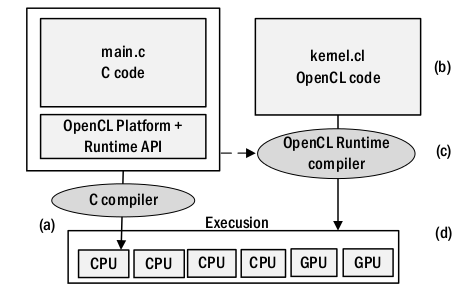
\includegraphics[scale=0.6]{OpenCL.png}
	\caption{OpenCL execution}
	\label{fig:OpenCL}
\end{figure}

The experiment in the paper uses DCT (discrete cosine transform). This is
basically large 2D matrix data computations. The paper implements four
different serial DCT versions: (1) implemented directly with serial processing,
(2) with precomputing coefficients, (3) based on (2) but using direct matrix
multiplication and (4) is the implementation of row-column decomposition
method. Another input variable is the matrix size, which is 256, 512, 1024 or
2048. For performance benchmarking the paper used TBB and OpenCL\@. From the
results we see that the OpenCL implementation outperforms the one on TBB\@.
For the parallel DTC implementations the speedup compared to the serial ones
are 4.8 and 6.9 times for TBB and OpenCL, respectively. Especially it shows
linear speedup, as the increase of 2D data sets.




\subsection{Data Parallel Programming Model for Many-Core Architectures}

The paper \emph{Data Parallel Programming Model for Many-Core Architectures}
\cite{ZhangDataParallelProgramming} by Yongpeng Zhang, written in 2011,
describes a data streaming framework on GPUs.

GPUs have proved successful providing significant performance gains by
exploiting data parallelism in existing algorithms. Programmers however are
used to writing sequential programs. The paper proposes a framework GStream,
a general-purpose, scalable data streaming framework on GPUs.

The amount of data that has to be processed continues to grow. However
Processor frequencies have reached their limits. Traditional instruction level
parallelism can no longer provide worthy performance benefits. A higher degree
of parallelism has to be extracted, both in algorithmic or implementation
level, to fully utilize emerging multi and many-core architectures.

Massive data-parallelization on the GPU can already be achieved with the NVIDIA
GPU programming model CUDA\@. CUDA encourages users to create light-weight
software threads at scale of thens of thousands, which is magnitudes larger
than the maximum hardware concurrency inside the GPU\@. Although CUDA has great
performance benefits, it requires deep understanding of the underlying
architecture. Therefore it is desirable to develop a new programming model to
reach an acceptable balance between programmability, portability and
performance that accommodate the increasing number of cores per chip.

The paper looks at the possibilities of the stream processing domain. Usually
used in video encoding/decoding scenarios. Other domains such as data analysis
and computationally intensive tasks are also discovering the benefits of the
underlying streaming paradigm. The GStream streaming framework developed by the
authors contributes the following: (1) abstraction expresses data-parallelism
more naturally than task-oriented parallelism, (2) extreme concise and
intuitive abstraction, (3) data-parallel approach reduces data dependencies,
(4) first work to exploit streaming applications on clusters of GPUs, (5) the
validity of the abstraction reaches beyond streaming.

Two key concepts of GStream are \emph{filter} and \emph{channels}. A filter
encapsulates the computing kernels that can be accelerated by the GPU\@. The
data-parallelism inherently to filter kernels is facilitated by simple APIs to
manipulate data in channels, which represent data links between any two
filters.

\begin{figure}[!h]
	\centering
	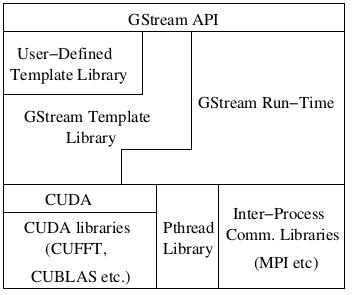
\includegraphics[scale=0.6]{GStreamStack.png}
	\caption{GStream Software Stack}
	\label{fig:GStreamStack}
\end{figure}

Figure~\ref{fig:GStreamStack} describes the GStream Software stack.
It uses CUDA for data-parallelism and POSIX threads for task-parallelism. None
of the concrete components are mandatory, as long as they are replaced with a
library with the same functionality.

The paper tested the acceleration by the GStream library with five benchmarks.
Using four different implementations: (a) A native single-threaded C/C++
program; (b) a multi-threaded C/C++ program using the GStream library without
GPU support; (c) a multi-threaded program using GStream with GPU support and
(d) a native CUDA implementation.

For three of the five benchmark applications the speedup is between 3 and 30
times. Comparing implementations (a) with (b) and (c) with (d) shows that the
GStream imposes little overhead to the overall system.




\section{Comparison}

% definition of evaluation and comparison criteria
% both quantitative nd qualitative

% results of comparison including thorough argumentation of pros and cons of
% the different approaches

For comparison and evaluation of different kinds of parallel programming
models there are a few criteria.

\begin{itemize}
	\item \textbf{Efficient exploitation of all the hardware:} If there are N
		cores in a processor, how well does the programming model use all the N
		cores, using good scheduling, load balancing and memory management.
	\item \textbf{Ease of use for programmers:} As utilizing all hardware is
		very difficult to do manually, programming models and frameworks can
		help to make it easier for programmers. Also how the
		method is implemented in the programming language, as pragmas, language
		extensions or library APIs is of importance to the learning curve and maintainability.
	\item \textbf{Scaling:} Can the solution be used on different
		architectures, how does it scale to many-core processors? Does it only
		work on CPUs or also GPUs, DSPs or even across a cluster.
\end{itemize}

\paragraph{Performance} \cite{CaoPerformanceAnalysis} presents a good
comparison for how the Cilk, TBB and OpenML programming models scale to more
cores. Each programming model is tested with different benchmarks so it's
difficult to actually compare the actual speedup ratios. What's also visible is
that the speedups become less when the number of cores increase, which can be
explained by Amdahls's Law \cite{hennessy2007computer}. OpenCL and TBB are
compared in \cite{KimExploitingMultiManyCore} with a discrete cosine transform
application, this paper focusses on computations on the GPU, which shows that
for that application the OpenCL method performs better than TBB.
\cite{BrightwellParallelPhaseModel} compares MPI with PPM for clusters of
multi-core machines and shows that the PPM is comparable in performance.
Finally \cite{ZhangDataParallelProgramming} presents GStream and does a
performance comparison between GStream and CUDA for GPUs and show that the
difference in performance between the two is in fact very small.

\paragraph{Ease of use} Especially \cite{BrightwellParallelPhaseModel} focusses
on the ease of use for parallel programming. It compares their PPM solution
with the message passing model MPI and get a substantial reduction of code size
of the same problem (as shown in table~\ref{tab:code-size}). It adds extra
declarations to the C programming language and needs an extra source-to-source
compiling step. TBB described in
\cite{KimExploitingMultiManyCore,CaoPerformanceAnalysis} is a C++ library and
does not need special languages or compilers. It is not further described if
using TBB tends to be easy or difficult. Cilk adds three keywords to the
programming language and aims for simplicity \cite{KimExploitingMultiManyCore}.
Simplicity is also an aim of OpenMP \cite{KimExploitingMultiManyCore}. Besides
\cite{BrightwellParallelPhaseModel} the other papers don't provide any metrics
that support claims about some method being easy to use for programmers or not.

\paragraph{Scaling} One of the reasons of the programming models
described in the four papers is that they can abstract platform specific
things. For example GStream's architecture (figure~\ref{fig:GStreamStack}) can
use CUDA, but the concrete implementation can be exchanged for something else,
so it is not NVIDIA dependent anymore \cite{ZhangDataParallelProgramming}.
Also the programmer doesn't have to think about the number of actual cores
anymore, because that's somewhere the programming model can manage. Between
the papers is a difference that \cite{BrightwellParallelPhaseModel} describes
an model that even generalizes over physical machines to a network cluster
using an intelligent allocation mechanism. For user applications this is
slightly more costly on a lower amount of cores but pays off when the number of
cores approaches 100 or more.  There the programmer does not need to worry
about which node and core does the computation, only that the computation
kernel should be parallelized. Other programming models like GStream and OpenCL
focus more on GPUs \cite{KimExploitingMultiManyCore,
ZhangDataParallelProgramming}.

\section{Conclusion}

We've identified a kernel function and changed the x264 program so the kernel
is executed on the \rvex. The kernel we used is the \satd function. Using our
abstracted \texttt{rvex*} functions you can write the instruction memory, write
and read the data memory and start the \rvex. Unfortunately we didn't see a
speedup, instead we even saw a decrease in performance. Assumably this is
because of the communication overhead. The \satd function is called many times.
Maybe by sending more data at once, and thus executing the \rvex less times
might improve the performance.

Using our \texttt{rvex*} functions, we were able to create different test
programs which helped us testing the communication and get to know the
platform, getting the endianness right and fixing multiple executions of the
\rvex.

All in all the lab was definitely fun. It felt really rewarding to hack
something together, inject some bytecode and see it working.

Regarding the results, we have some suggestions that we would have tried out
given enough time.

We still believe in the \rvex{} so we would try to reduce the performance loss
of the current bottleneck: communication. This can be done by reducing the
number of reads and writes to the \rvex{}. This means selecting a bigger part
of the application and send it over to the \rvex{} in its entirety.

We are interested in if the \rvex{} performance is dependent on the type of
program that is run. Is it more efficient for highly repeating code or does it
perform just as well for dynamic code with little repetition compared to the
normal CPUs?



\bibliographystyle{plain}
\bibliography{main}

\end{document}

